\section{Physics}

\begin{frame}{Physics setup}
	\begin{block}{Lagrangian}
	\begin{equation*}\label{eq:Lbc}
	\mathcal{L}_\text{eff} = -\frac{4G_F}{\sqrt{2}}V_{cb}\left[C_{VL}O_{VL}+C_{VR}O_{VR}+C_{SL}O_{SL}+C_{SR}O_{SR}+C_{T}O_{T}\right]+\text{h.c.}
	\end{equation*}
	with the effective operators
	%
	\begin{align*}
	O_{VL}&= (\bar c \gamma_\mu P_L b)(\bar \tau \gamma^\mu P_L \nu_\tau)\,, &  O_{VR}&= (\bar c \gamma_\mu P_R \,b)(\bar \tau \gamma^\mu P_L \nu_\tau)\,,\notag\\
	O_{SL}&= (\bar c P_L b)(\bar \tau  P_L \nu_\tau)\,,& O_{SR}&= (\bar c  P_R b)(\bar \tau  P_L \nu_\tau)\,, \\
	O_{T}&= (\bar c \sigma_{\mu\nu} P_L b)(\bar \tau \sigma^{\mu\nu} P_L \nu_\tau)\,. &\notag
	\end{align*} 
	where $P_{R,L}=\frac{1}{2}(1\pm\gamma_5)$, $\sigma^{\mu\nu}=\frac{\mathrm i}{2}[\gamma^\mu,\gamma^\nu]$
	
	\end{block}
	\begin{block}{Assumptions}
	\begin{itemize}
		\item $CP$ conserving limit $\Lra$ real Wilson coeffs
		\item Presentational reasons: Consider $C_{VL}$, $C_{SL}$, $C_T$
		\item $C_T$ is constrained from longitudinal polarization fraction $F_L$ $\Lra$ $C_T\in [-0.1, 0.1]$
		\item $C_{VL}, C_{SL}\in [-0.5, 0.5]$
	\end{itemize}
	\end{block}
\end{frame}

\begin{frame}{Observables}
	We now look at several observables of $\mathrm{BR}(B\to D^{0*} \tau\nu)$
	\begin{itemize}
		\item \hhl{$\theta_\tau$}: angle between the $\tau$ and the $B$ meson in the dilepton mass frame
		\item \hhl{$\theta_V$}: angle between $D^{0*}$ and $B$ meson
		\item \hhl{$q^2$}: mass transfer $(p_B-p_{D^*})^2=(p_\tau+p_\nu)^2$
		\item \hhl{$E_l$}: energy of the light lepton $\ell$ from the 5-body decay $\bar B\to D \tau^-(\to\ell\, \bar\nu_\ell\,\nu_\tau)\bar\nu_\tau$
	\end{itemize}

	If not stated otherwise, we assign Poisson uncertainties corresponding to a yield of \hhl{700} and \hhl{$1\%$ relative uncertainties} (uncorrelated)
\end{frame}

\begin{frame}{$\cos\theta_\tau$}{2D cuts of clustered parameter space}
	%\vspace{-0.3cm}
	\begin{changemargin}{-1cm}{-1cm}
		\centering
		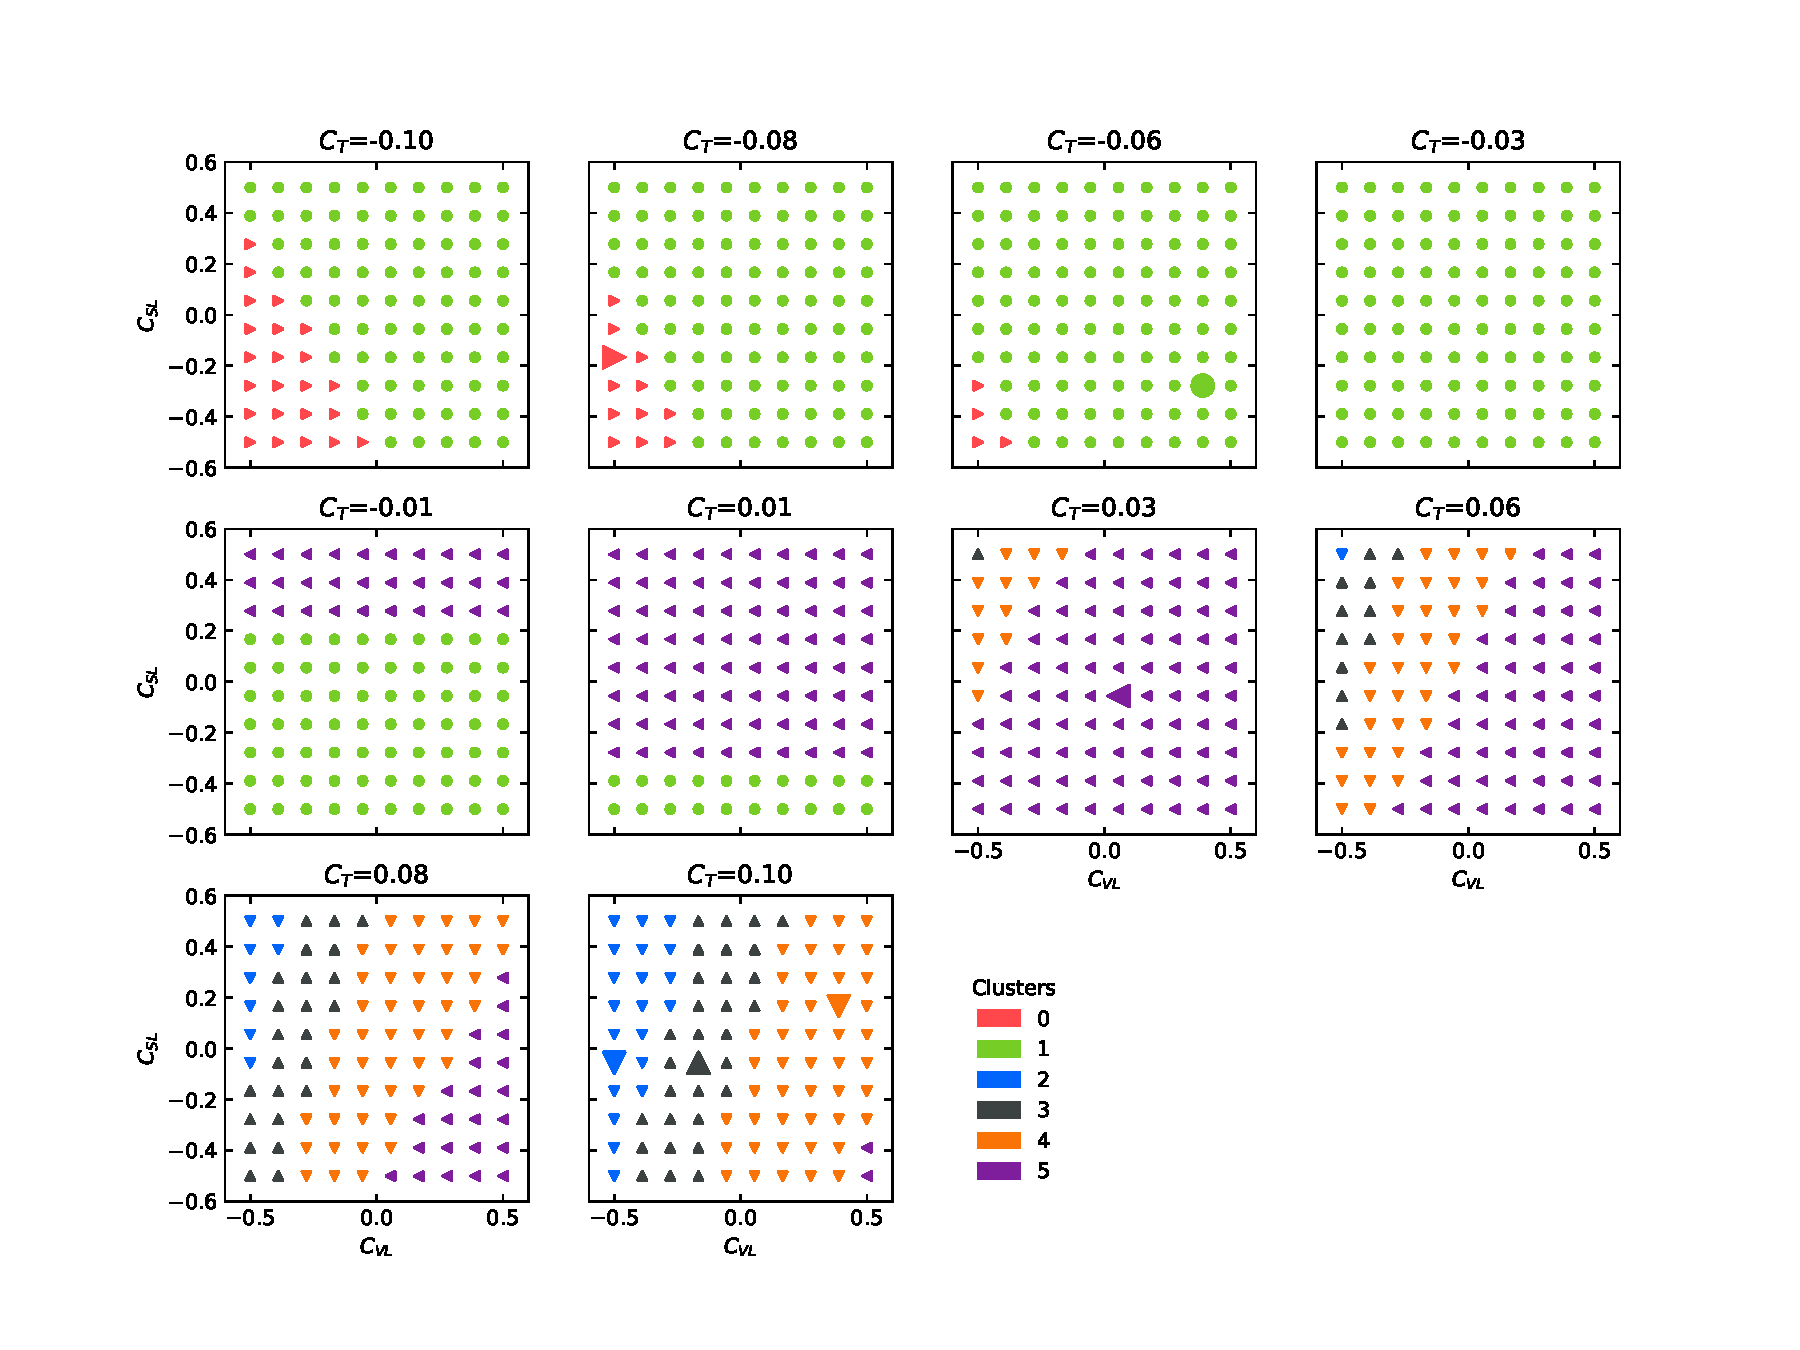
\includegraphics[width=12.5cm,clip,trim=0cm 0cm 0cm 2cm]{figures/from-paper/cosl_clust2D.pdf}
	\end{changemargin}
\end{frame}
%
\begin{frame}{$\cos\theta_\tau$}{The distributions}
	\centering
%	\begin{figure}
	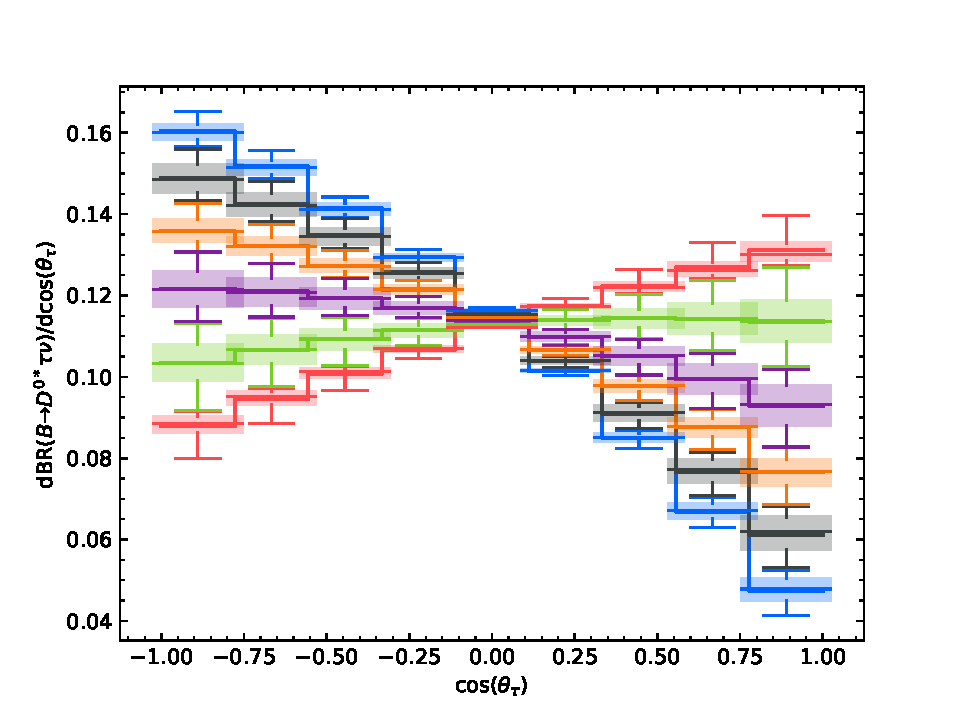
\includegraphics[width=8cm, clip, trim=1cm 0.75cm 1cm 1cm]{figures/from-paper/cosl_box.pdf}
	
	Distribution of bin contents for curves of different clusters;\\
	benchmark curves solid lines \srem{(looking reasonable)}
	
	%\label{nolabel}
%	\end{figure}
\end{frame}
%
\begin{frame}{$\cos\theta_V$}
	\centering
	3 clusters, but distinct shape from previous ones
	\begin{changemargin}{-1cm}{-1cm}
		{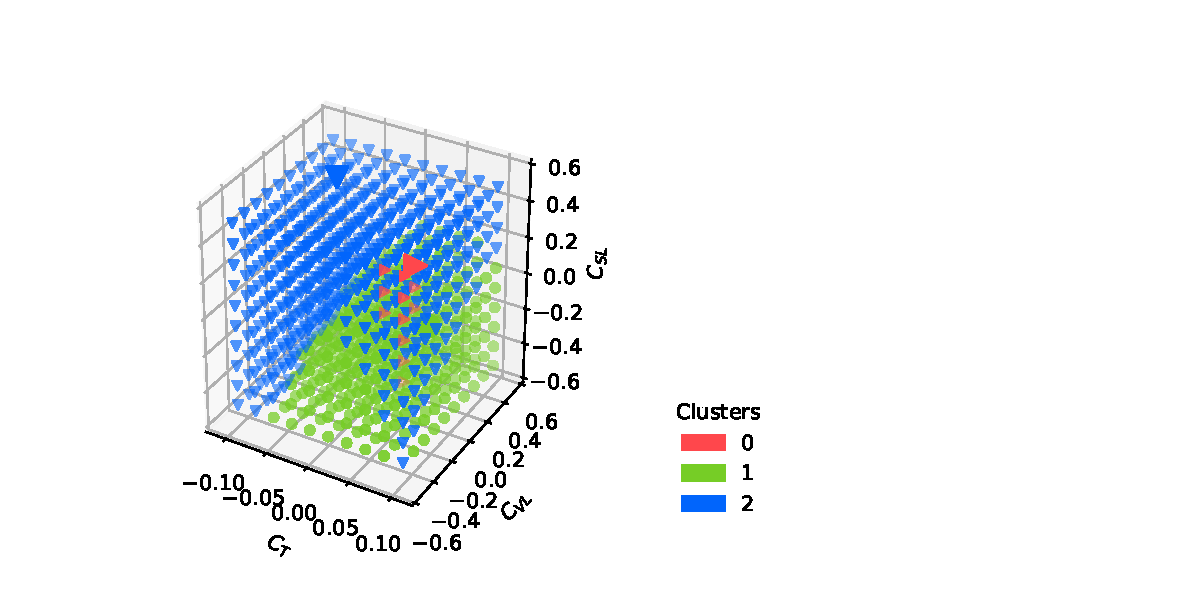
\includegraphics[width=5cm,clip,trim=3cm 0.3cm 7.5cm 1cm]{figures/from-paper/cosV_3D.pdf}}
		{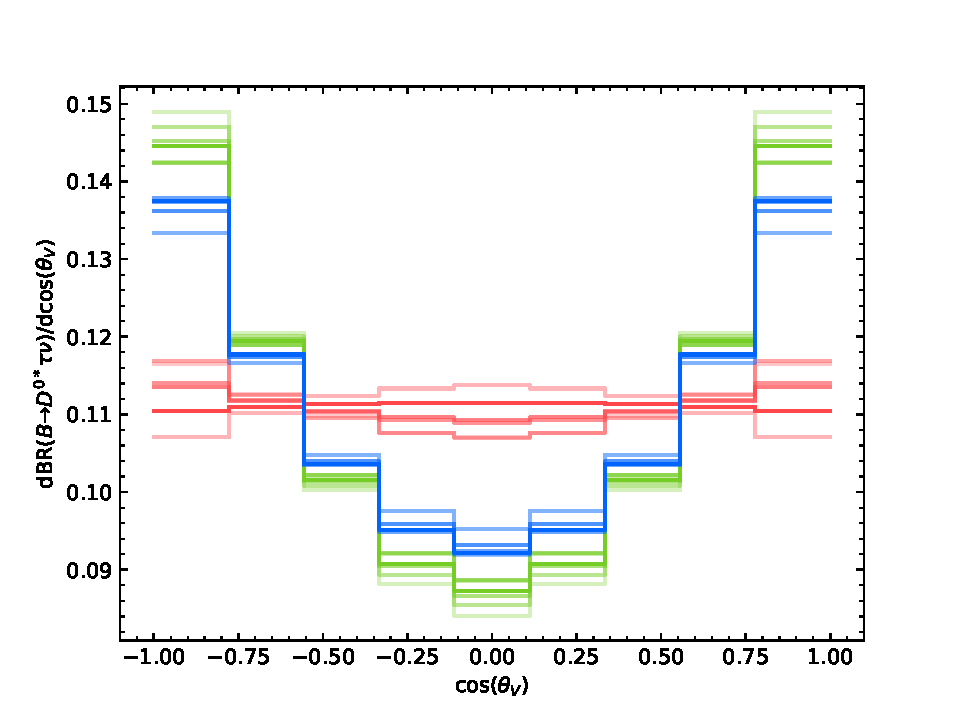
\includegraphics[width=7cm,clip,trim=0.3cm 0.cm 1.5cm 0cm]{figures/from-paper/cosV_dist.pdf}}
	\end{changemargin}
\end{frame}
%
\begin{frame}{$q^2$}{Number of clusters vs yield and systematic uncertainties}
	\centering
	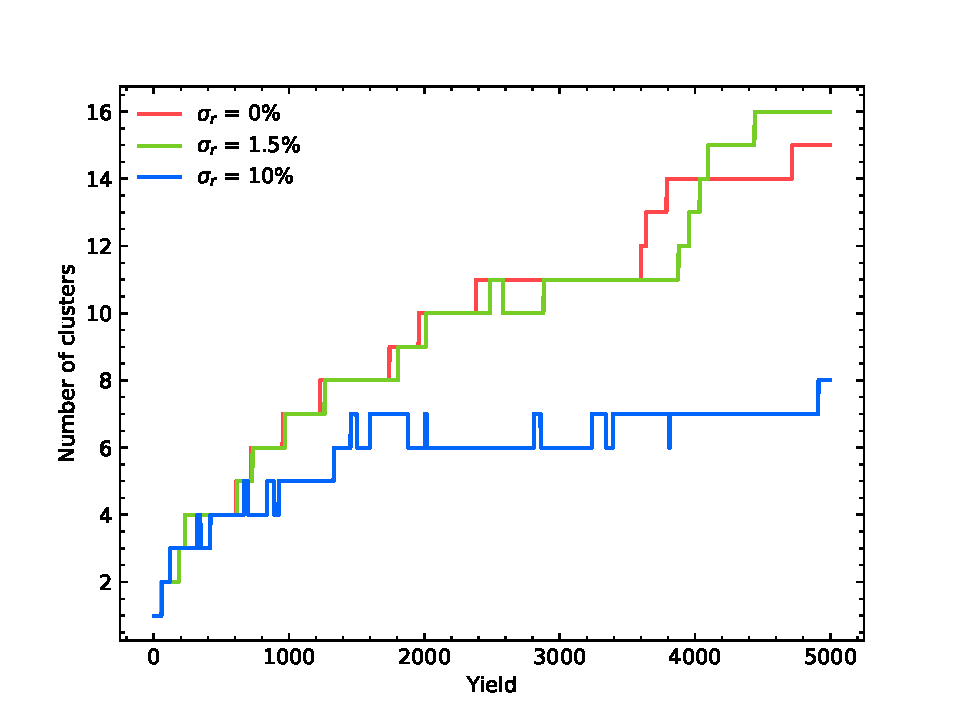
\includegraphics[width=10cm]{figures/from-paper/clust_yield.pdf}
	% validate: Rel uncertinaties irrelevant for very low yields
	% stat uncertainty irrelevant for very high yields (dominated syst)
\end{frame}
%
\begin{frame}{$E_\ell$}
	\centering
	\begin{changemargin}{-1cm}{-1cm}
	{
		\begin{minipage}{10cm}
			\centering
			{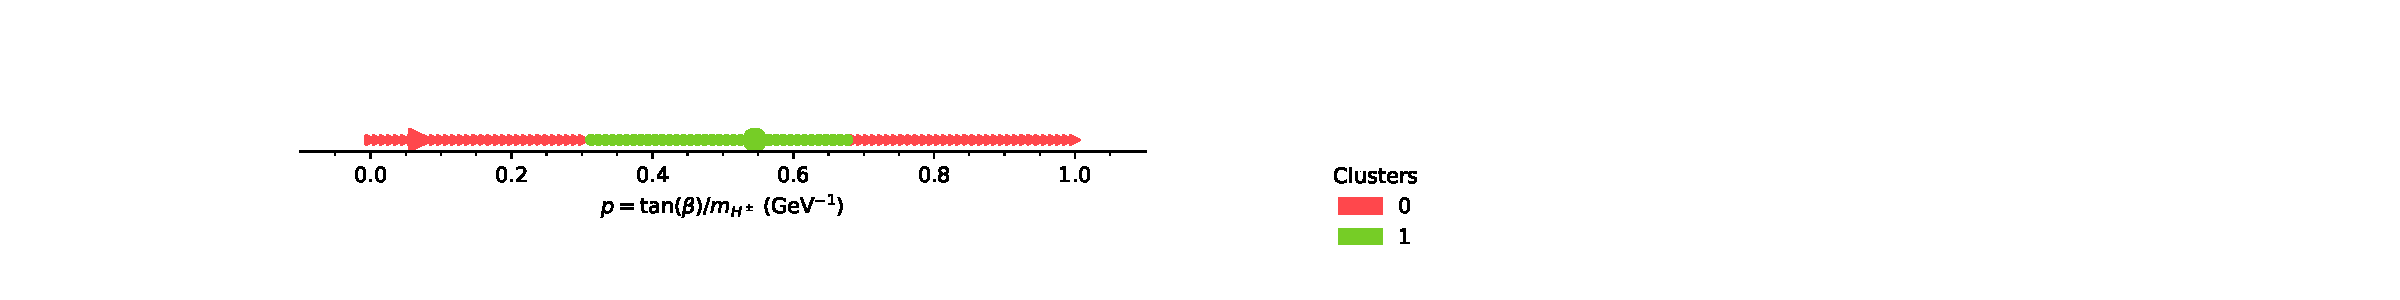
\includegraphics[clip, trim=4.5cm 1cm 21cm 2.0cm, height=1.3cm]{figures/from-paper/El_tanbeta_err1}}
			{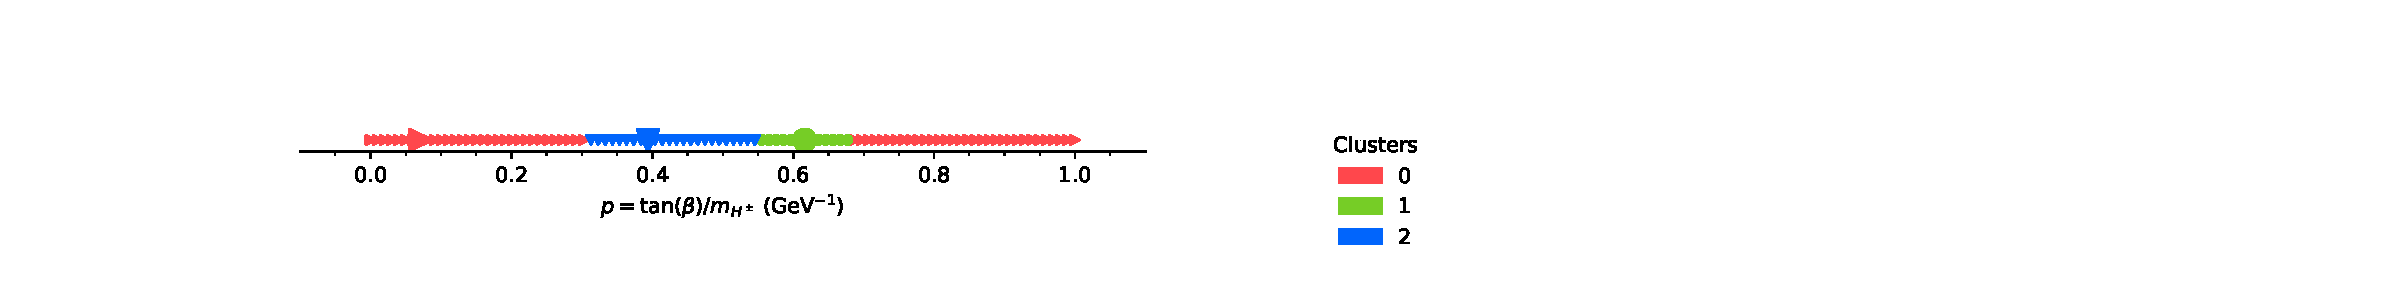
\includegraphics[clip, trim=4.5cm 1cm 21cm 2.0cm, height=1.3cm]{figures/from-paper/El_tanbeta_err2}}
			{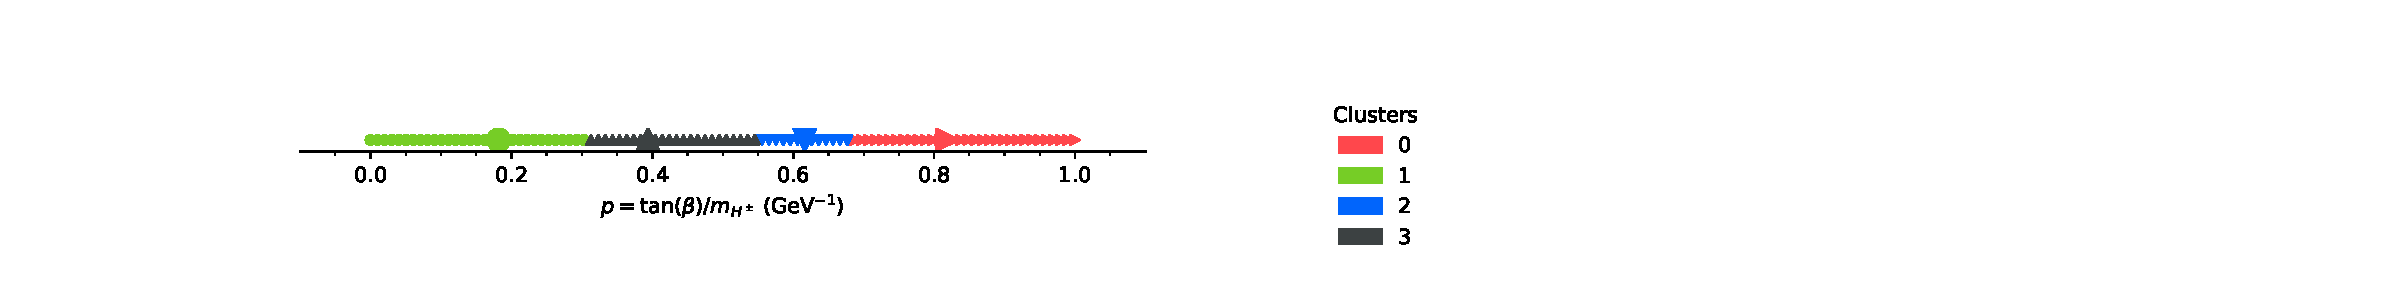
\includegraphics[clip, trim=4.5cm 1cm 21cm 2.0cm, height=1.3cm]{figures/from-paper/El_tanbeta_err3}}
	\end{minipage}
	}
	\begin{minipage}{2cm}
		\vspace{2cm}
		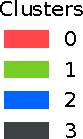
\includegraphics[height=1.7cm]{figures/from-paper/el_err3_legend.pdf}
	\end{minipage}
	\end{changemargin}
\end{frame}

\begin{frame}{$E_\ell$}
	\begin{changemargin}{-1cm}{-1cm}
		\begin{center}
			{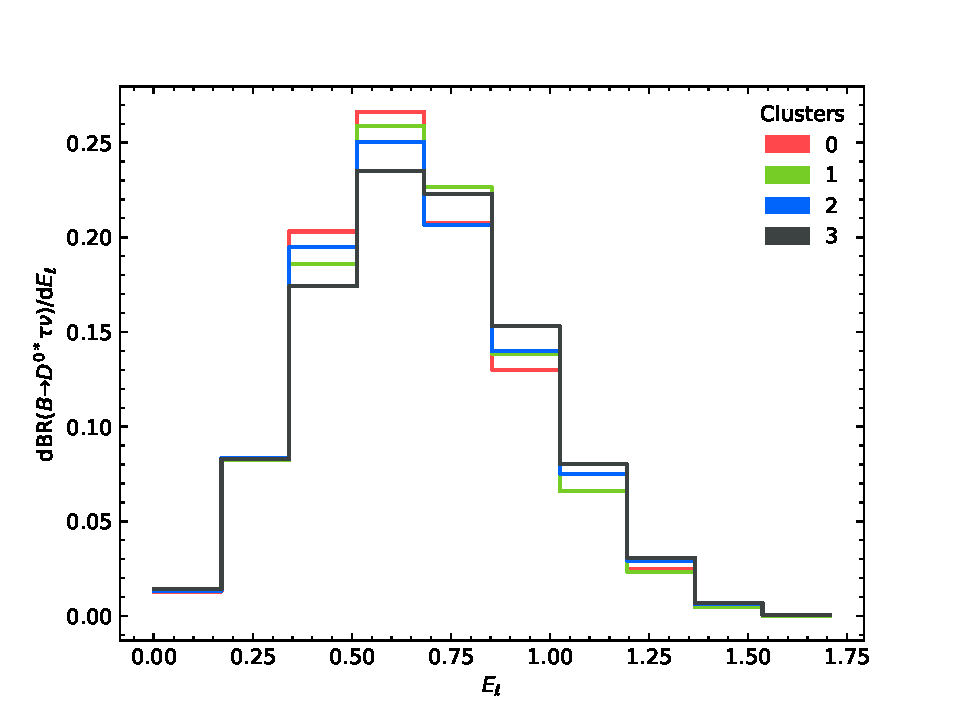
\includegraphics[height=5.2cm, clip, trim=0cm 0cm 1.2cm 1cm]{figures/from-paper/El_tanbeta_dist3}}
			{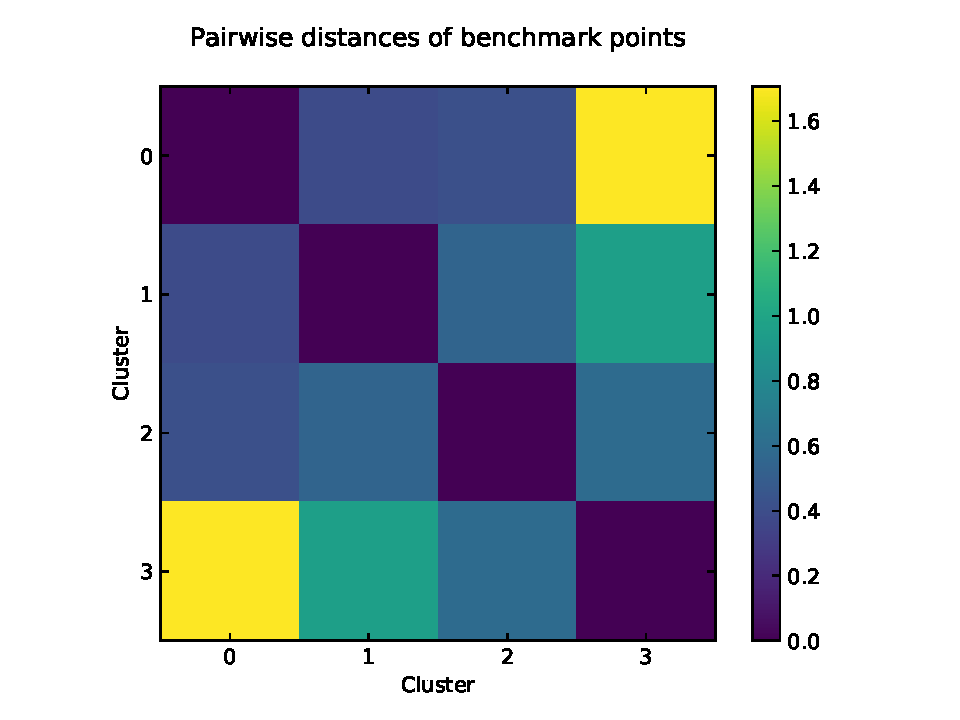
\includegraphics[height=5.2cm, clip, trim=2.3cm 0cm 2cm 0cm]{figures/from-paper/El_tanbeta_dist3_bpoint_distances}}
		\end{center}
	\end{changemargin}
\end{frame}